\documentclass{standalone}
\author{Quinten Bruynseraede}
\usepackage{tikz}
\usetikzlibrary{shapes}
\title{Tikz grafen}
\begin{document}\pagestyle{empty}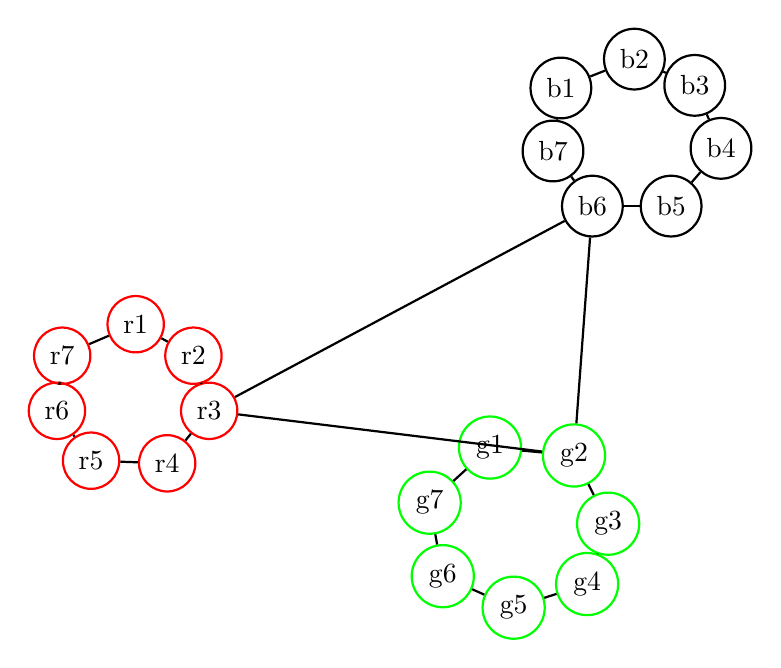
\begin{tikzpicture}\node[shape=circle,draw=red,align=center,line width=0.8pt] (0) at (1.5666666666666667,9.9) {r6};
\node[shape=circle,draw=red,align=center,line width=0.8pt] (1) at (1.6333333333333333,10.6) {r7};
\node[shape=circle,draw=red,align=center,line width=0.8pt] (2) at (2.566666666666667,11.0) {r1};
\node[shape=circle,draw=red,align=center,line width=0.8pt] (3) at (3.3,10.6) {r2};
\node[shape=circle,draw=red,align=center,line width=0.8pt] (4) at (3.5,9.9) {r3};
\node[shape=circle,draw=red,align=center,line width=0.8pt] (5) at (2.966666666666667,9.233333333333333) {r4};
\node[shape=circle,draw=red,align=center,line width=0.8pt] (6) at (2.0,9.266666666666667) {r5};
\node[shape=circle,draw=black,align=center,line width=0.8pt] (7) at (7.966666666666667,14.0) {b1};
\node[shape=circle,draw=black,align=center,line width=0.8pt] (8) at (8.9,14.366666666666667) {b2};
\node[shape=circle,draw=black,align=center,line width=0.8pt] (9) at (9.666666666666666,14.033333333333333) {b3};
\node[shape=circle,draw=black,align=center,line width=0.8pt] (10) at (10.0,13.233333333333333) {b4};
\node[shape=circle,draw=black,align=center,line width=0.8pt] (11) at (9.366666666666667,12.5) {b5};
\node[shape=circle,draw=black,align=center,line width=0.8pt] (12) at (8.366666666666667,12.5) {b6};
\node[shape=circle,draw=black,align=center,line width=0.8pt] (13) at (7.866666666666666,13.2) {b7};
\node[shape=circle,draw=green,align=center,line width=0.8pt] (14) at (6.3,8.733333333333333) {g7};
\node[shape=circle,draw=green,align=center,line width=0.8pt] (15) at (7.066666666666666,9.433333333333334) {g1};
\node[shape=circle,draw=green,align=center,line width=0.8pt] (16) at (8.133333333333333,9.333333333333334) {g2};
\node[shape=circle,draw=green,align=center,line width=0.8pt] (17) at (8.566666666666666,8.466666666666667) {g3};
\node[shape=circle,draw=green,align=center,line width=0.8pt] (18) at (8.3,7.7) {g4};
\node[shape=circle,draw=green,align=center,line width=0.8pt] (19) at (7.366666666666666,7.4) {g5};
\node[shape=circle,draw=green,align=center,line width=0.8pt] (20) at (6.466666666666667,7.8) {g6};

\path [-,draw=black,line width=0.8pt] (1) edge node {} (2);
\path [-,draw=black,line width=0.8pt] (2) edge node {} (3);
\path [-,draw=black,line width=0.8pt] (3) edge node {} (4);
\path [-,draw=black,line width=0.8pt] (4) edge node {} (5);
\path [-,draw=black,line width=0.8pt] (5) edge node {} (6);
\path [-,draw=black,line width=0.8pt] (6) edge node {} (0);
\path [-,draw=black,line width=0.8pt] (0) edge node {} (1);
\path [-,draw=black,line width=0.8pt] (15) edge node {} (16);
\path [-,draw=black,line width=0.8pt] (16) edge node {} (17);
\path [-,draw=black,line width=0.8pt] (17) edge node {} (18);
\path [-,draw=black,line width=0.8pt] (18) edge node {} (19);
\path [-,draw=black,line width=0.8pt] (19) edge node {} (20);
\path [-,draw=black,line width=0.8pt] (20) edge node {} (14);
\path [-,draw=black,line width=0.8pt] (14) edge node {} (15);
\path [-,draw=black,line width=0.8pt] (7) edge node {} (8);
\path [-,draw=black,line width=0.8pt] (8) edge node {} (9);
\path [-,draw=black,line width=0.8pt] (9) edge node {} (10);
\path [-,draw=black,line width=0.8pt] (10) edge node {} (11);
\path [-,draw=black,line width=0.8pt] (11) edge node {} (12);
\path [-,draw=black,line width=0.8pt] (12) edge node {} (13);
\path [-,draw=black,line width=0.8pt] (13) edge node {} (7);
\path [-,draw=black,line width=0.8pt] (12) edge node {} (16);
\path [-,draw=black,line width=0.8pt] (12) edge node {} (4);
\path [-,draw=black,line width=0.8pt] (4) edge node {} (16);
\end{tikzpicture}
\end{document}